\subsubsection{Wi-Fi}

Wi-Fi (\textit{Wireless Fidelity}) es un conjunto de tecnologías que permiten la comunicación inalámbrica entre dispositivos electrónicos utilizando ondas electromagnéticas. Es uno de los protocolos de comunicación más comunes en redes locales (WLAN) y se basa en la familia de estándares IEEE 802.11 \cite{ieee_802.11}, desarrollados y mantenidos por el Instituto de Ingenieros Eléctricos y Electrónicos (IEEE). Wi-Fi es ampliamente utilizado en aplicaciones que requieren conectividad a internet o comunicación local sin cables, lo que lo convierte en una opción clave en proyectos de IoT y sistemas embebidos. \\


Wi-Fi opera en bandas de frecuencia de 2.4 GHz y 5 GHz, y permite a los dispositivos conectarse a una red a través de un punto de acceso (\textit{Access Point}) o funcionar en un modo de conexión directa \textit{peer-to-peer} (ad-hoc). En la figura \ref{fig:wifi} se visualizan los dos tipos de conexiones mencionadas. En un entorno típico, un \textit{router} actúa como el punto de acceso central, al cual se conectan varios dispositivos para intercambiar datos entre sí y acceder a internet. \\ 

\begin{figure}[H]
    \centering
    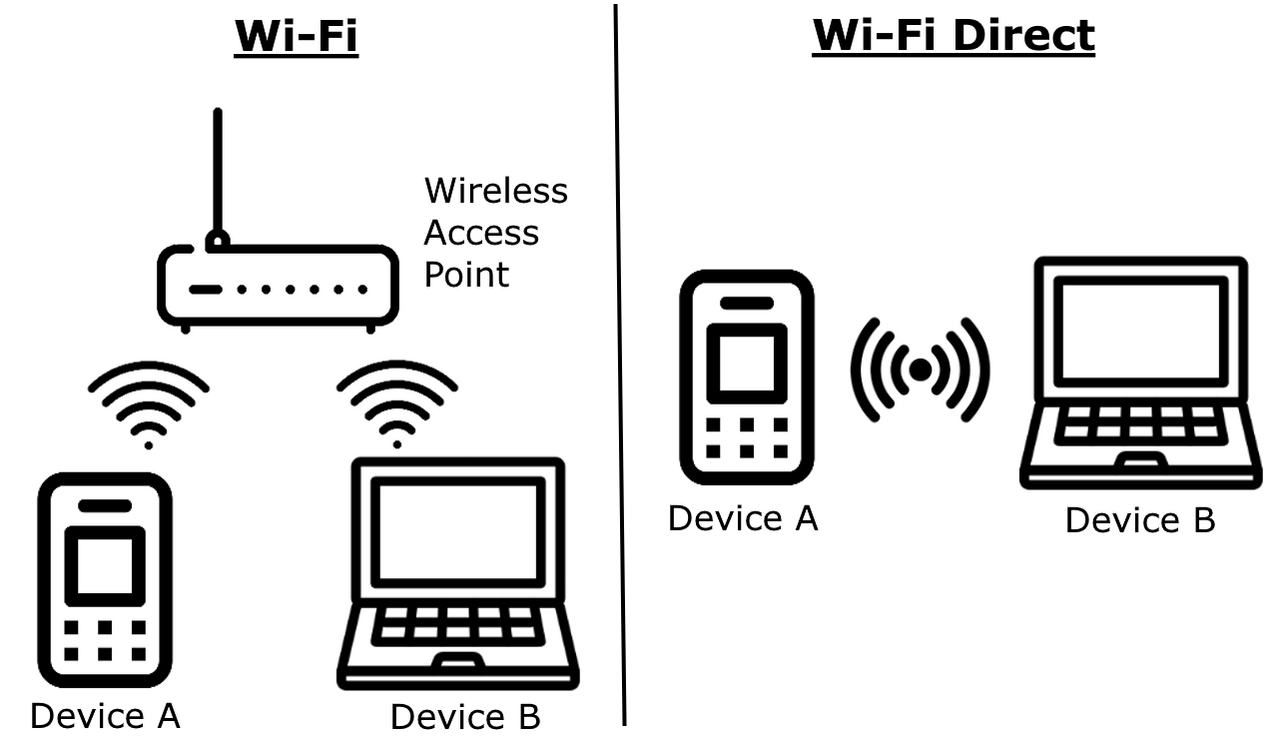
\includegraphics[width = 0.7 \linewidth]{img/wifi.png}
    \caption{Modos de conexión Wi-Fi \cite{wifi_img}}
    \label{fig:wifi}
\end{figure}


Las principales características de Wi-Fi son las siguientes:

\begin{itemize}
    \item \textbf{Alcance}: Ofrece un rango de cobertura considerable, que generalmente varía entre 20 a 50 metros en interiores y hasta 100 metros en exteriores, dependiendo de las condiciones de señal y el entorno.
    
    \item \textbf{Velocidad}: Permite transmitir datos a distintas velocidades según la señal y las condiciones de la red, ofreciendo un rendimiento adecuado para la mayoría de las aplicaciones cotidianas.
    
    \item \textbf{Seguridad}: Incorpora varios protocolos de seguridad, como WEP, WPA y WPA2 \cite{wifi_security}, que aseguran la comunicación cifrada entre dispositivos y protegen las redes inalámbricas de accesos no autorizados.
    
    \item \textbf{Compatibilidad}: Es retrocompatible, lo que significa que los dispositivos más antiguos que soportan versiones previas del estándar, como 802.11a, b, g o n, pueden seguir conectándose a redes más modernas, aunque con limitaciones en velocidad y funcionalidad.
    
   
\end{itemize}






El protocolo Wi-Fi cuenta con algunas limitaciones como su consumo de energía; que suele ser mayor comparado con otros protocolos con el Bluetooth, o la congestión y colisiones que pueden ocurrir en entornos densos con muchos dispositivos conectados; esto puede generar interferencia y degradación en el rendimiento de las conexiones. \\

Sin embargo, el Wi-FI se popularizó cada vez más debido las siguientes ventajas que genera:

\begin{itemize}
    
    \item \textbf{Flexibilidad}: Elimina la necesidad de cables, lo que facilita la instalación y operación en entornos móviles o de difícil acceso. Esto es especialmente útil en redes IoT donde se requiere la conectividad de múltiples dispositivos dispersos.

    
    \item \textbf{Conectividad global}: La mayoría de los dispositivos modernos, desde teléfonos móviles hasta microcontroladores y computadoras, tienen Wi-Fi integrado, lo que permite la interoperabilidad entre diferentes plataformas y tecnologías.

    \item \textbf{Alta velocidad de transmisión}: Es adecuado tanto para aplicaciones que requieren grandes volúmenes de datos, como la transmisión de video en tiempo real, como para aquellas que necesitan una transferencia rápida, como la telemetría o la comunicación de sensores.
\end{itemize}


Wi-Fi es el protocolo preferido para aplicaciones que requieren transferencias rápidas y confiables de datos, como transmisión de video, comunicación entre dispositivos móviles, automatización del hogar y acceso a internet en redes locales. También es fundamental en muchas aplicaciones de IoT que requieren conectividad en tiempo real y de alto ancho de banda.